% Options for packages loaded elsewhere
\PassOptionsToPackage{unicode}{hyperref}
\PassOptionsToPackage{hyphens}{url}
\PassOptionsToPackage{dvipsnames,svgnames,x11names}{xcolor}
%
\documentclass[
  xelatex,
  ja=standard]{bxjsarticle}

\usepackage{amsmath,amssymb}
\usepackage{iftex}
\ifPDFTeX
  \usepackage[T1]{fontenc}
  \usepackage[utf8]{inputenc}
  \usepackage{textcomp} % provide euro and other symbols
\else % if luatex or xetex
  \usepackage{unicode-math}
  \defaultfontfeatures{Scale=MatchLowercase}
  \defaultfontfeatures[\rmfamily]{Ligatures=TeX,Scale=1}
\fi
\usepackage{lmodern}
\ifPDFTeX\else  
    % xetex/luatex font selection
  \setmainfont[BoldFont=Noto Sans CJK JP]{Noto Serif CJK JP}
\fi
% Use upquote if available, for straight quotes in verbatim environments
\IfFileExists{upquote.sty}{\usepackage{upquote}}{}
\IfFileExists{microtype.sty}{% use microtype if available
  \usepackage[]{microtype}
  \UseMicrotypeSet[protrusion]{basicmath} % disable protrusion for tt fonts
}{}
\makeatletter
\@ifundefined{KOMAClassName}{% if non-KOMA class
  \IfFileExists{parskip.sty}{%
    \usepackage{parskip}
  }{% else
    \setlength{\parindent}{0pt}
    \setlength{\parskip}{6pt plus 2pt minus 1pt}}
}{% if KOMA class
  \KOMAoptions{parskip=half}}
\makeatother
\usepackage{xcolor}
\setlength{\emergencystretch}{3em} % prevent overfull lines
\setcounter{secnumdepth}{5}
% Make \paragraph and \subparagraph free-standing
\ifx\paragraph\undefined\else
  \let\oldparagraph\paragraph
  \renewcommand{\paragraph}[1]{\oldparagraph{#1}\mbox{}}
\fi
\ifx\subparagraph\undefined\else
  \let\oldsubparagraph\subparagraph
  \renewcommand{\subparagraph}[1]{\oldsubparagraph{#1}\mbox{}}
\fi


\providecommand{\tightlist}{%
  \setlength{\itemsep}{0pt}\setlength{\parskip}{0pt}}\usepackage{longtable,booktabs,array}
\usepackage{calc} % for calculating minipage widths
% Correct order of tables after \paragraph or \subparagraph
\usepackage{etoolbox}
\makeatletter
\patchcmd\longtable{\par}{\if@noskipsec\mbox{}\fi\par}{}{}
\makeatother
% Allow footnotes in longtable head/foot
\IfFileExists{footnotehyper.sty}{\usepackage{footnotehyper}}{\usepackage{footnote}}
\makesavenoteenv{longtable}
\usepackage{graphicx}
\makeatletter
\def\maxwidth{\ifdim\Gin@nat@width>\linewidth\linewidth\else\Gin@nat@width\fi}
\def\maxheight{\ifdim\Gin@nat@height>\textheight\textheight\else\Gin@nat@height\fi}
\makeatother
% Scale images if necessary, so that they will not overflow the page
% margins by default, and it is still possible to overwrite the defaults
% using explicit options in \includegraphics[width, height, ...]{}
\setkeys{Gin}{width=\maxwidth,height=\maxheight,keepaspectratio}
% Set default figure placement to htbp
\makeatletter
\def\fps@figure{htbp}
\makeatother

\renewcommand{\thefootnote}{\arabic{footnote}}
\makeatletter
\@ifpackageloaded{tcolorbox}{}{\usepackage[skins,breakable]{tcolorbox}}
\@ifpackageloaded{fontawesome5}{}{\usepackage{fontawesome5}}
\definecolor{quarto-callout-color}{HTML}{909090}
\definecolor{quarto-callout-note-color}{HTML}{0758E5}
\definecolor{quarto-callout-important-color}{HTML}{CC1914}
\definecolor{quarto-callout-warning-color}{HTML}{EB9113}
\definecolor{quarto-callout-tip-color}{HTML}{00A047}
\definecolor{quarto-callout-caution-color}{HTML}{FC5300}
\definecolor{quarto-callout-color-frame}{HTML}{acacac}
\definecolor{quarto-callout-note-color-frame}{HTML}{4582ec}
\definecolor{quarto-callout-important-color-frame}{HTML}{d9534f}
\definecolor{quarto-callout-warning-color-frame}{HTML}{f0ad4e}
\definecolor{quarto-callout-tip-color-frame}{HTML}{02b875}
\definecolor{quarto-callout-caution-color-frame}{HTML}{fd7e14}
\makeatother
\makeatletter
\makeatother
\makeatletter
\makeatother
\makeatletter
\@ifpackageloaded{caption}{}{\usepackage{caption}}
\AtBeginDocument{%
\ifdefined\contentsname
  \renewcommand*\contentsname{目次}
\else
  \newcommand\contentsname{目次}
\fi
\ifdefined\listfigurename
  \renewcommand*\listfigurename{図一覧}
\else
  \newcommand\listfigurename{図一覧}
\fi
\ifdefined\listtablename
  \renewcommand*\listtablename{表一覧}
\else
  \newcommand\listtablename{表一覧}
\fi
\ifdefined\figurename
  \renewcommand*\figurename{図}
\else
  \newcommand\figurename{図}
\fi
\ifdefined\tablename
  \renewcommand*\tablename{表}
\else
  \newcommand\tablename{表}
\fi
}
\@ifpackageloaded{float}{}{\usepackage{float}}
\floatstyle{ruled}
\@ifundefined{c@chapter}{\newfloat{codelisting}{h}{lop}}{\newfloat{codelisting}{h}{lop}[chapter]}
\floatname{codelisting}{コード}
\newcommand*\listoflistings{\listof{codelisting}{コード一覧}}
\makeatother
\makeatletter
\@ifpackageloaded{caption}{}{\usepackage{caption}}
\@ifpackageloaded{subcaption}{}{\usepackage{subcaption}}
\makeatother
\makeatletter
\@ifpackageloaded{tcolorbox}{}{\usepackage[skins,breakable]{tcolorbox}}
\makeatother
\makeatletter
\@ifundefined{shadecolor}{\definecolor{shadecolor}{rgb}{.97, .97, .97}}
\makeatother
\makeatletter
\makeatother
\makeatletter
\makeatother
\ifLuaTeX
\usepackage[bidi=basic]{babel}
\else
\usepackage[bidi=default]{babel}
\fi
\babelprovide[main,import]{japanese}
% get rid of language-specific shorthands (see #6817):
\let\LanguageShortHands\languageshorthands
\def\languageshorthands#1{}
\ifLuaTeX
  \usepackage{selnolig}  % disable illegal ligatures
\fi
\usepackage[]{natbib}
\bibliographystyle{jecon}
\IfFileExists{bookmark.sty}{\usepackage{bookmark}}{\usepackage{hyperref}}
\IfFileExists{xurl.sty}{\usepackage{xurl}}{} % add URL line breaks if available
\urlstyle{same} % disable monospaced font for URLs
\hypersetup{
  pdftitle={人権保障},
  pdfauthor={土井翔平},
  pdflang={ja},
  colorlinks=true,
  linkcolor={NavyBlue},
  filecolor={Maroon},
  citecolor={NavyBlue},
  urlcolor={NavyBlue},
  pdfcreator={LaTeX via pandoc}}

\title{人権保障}
\usepackage{etoolbox}
\makeatletter
\providecommand{\subtitle}[1]{% add subtitle to \maketitle
  \apptocmd{\@title}{\par {\large #1 \par}}{}{}
}
\makeatother
\subtitle{国際公共政策学}
\author{土井翔平}
\date{2023-07-18}

\begin{document}
\maketitle
\ifdefined\Shaded\renewenvironment{Shaded}{\begin{tcolorbox}[enhanced, sharp corners, interior hidden, boxrule=0pt, frame hidden, borderline west={3pt}{0pt}{shadecolor}, breakable]}{\end{tcolorbox}}\fi

\hypertarget{ux306fux3058ux3081ux306b}{%
\section*{はじめに}\label{ux306fux3058ux3081ux306b}}
\addcontentsline{toc}{section}{はじめに}

17-18世紀の啓蒙思想家\(\leadsto\)人が生まれながらにして持っている\textbf{自然権}
(natural rights)

\begin{tcolorbox}[enhanced jigsaw, rightrule=.15mm, opacitybacktitle=0.6, colback=white, bottomrule=.15mm, colbacktitle=quarto-callout-note-color!10!white, left=2mm, opacityback=0, toprule=.15mm, titlerule=0mm, bottomtitle=1mm, toptitle=1mm, colframe=quarto-callout-note-color-frame, title=\textcolor{quarto-callout-note-color}{\faInfo}\hspace{0.5em}{アメリカ独立宣言(1776年)}, arc=.35mm, breakable, leftrule=.75mm, coltitle=black]

われわれは、以下の事実を自明のことと信じる。すなわち、すべての人間は\textbf{生まれながらにして平等}であり、その創造主によって、生命、自由、および幸福の追求を含む\textbf{不可侵の権利}を与えられているということ。

\end{tcolorbox}

\begin{tcolorbox}[enhanced jigsaw, rightrule=.15mm, opacitybacktitle=0.6, colback=white, bottomrule=.15mm, colbacktitle=quarto-callout-note-color!10!white, left=2mm, opacityback=0, toprule=.15mm, titlerule=0mm, bottomtitle=1mm, toptitle=1mm, colframe=quarto-callout-note-color-frame, title=\textcolor{quarto-callout-note-color}{\faInfo}\hspace{0.5em}{フランス人権宣言(1789年)}, arc=.35mm, breakable, leftrule=.75mm, coltitle=black]

フランス人権宣言 人は、\textbf{自由かつ諸権利において平等なもの}として生まれ、そして生存する。

\end{tcolorbox}

\begin{itemize}
\tightlist
\item
  なぜ人権は保障されないのか?
\item
  なぜ他国の人権保障に関心を持つのか?
\item
  どのように国際的な人権保障に取り組んでいるのか?
\end{itemize}

\hypertarget{ux4ebaux6a29ux306eux56fdux969bux5316}{%
\section{人権の国際化}\label{ux4ebaux6a29ux306eux56fdux969bux5316}}

\hypertarget{ux7b2cux4e8cux6b21ux4e16ux754cux5927ux6226ux307eux3067}{%
\subsection{第二次世界大戦まで}\label{ux7b2cux4e8cux6b21ux4e16ux754cux5927ux6226ux307eux3067}}

人権問題=国内問題/主権国家体系の下で他国の国内問題に干渉することは\textbf{内政不干渉原則}?

\begin{itemize}
\tightlist
\item
  国家主権の契機となったウェストファリア条約

  \begin{itemize}
  \tightlist
  \item
    宗教戦争であった30年戦争
  \item
    領主の信仰の自由
  \end{itemize}
\item
  内政問題を口実とした戦争を回避するためのメカニズムとしての主権
\end{itemize}

\(\leadsto\)国家主権の下で人権侵害/国際社会からの批判をかわす口実

内政問題である人権問題に対して国際社会が無関心ではいられない?

\begin{itemize}
\tightlist
\item
  19世紀における奴隷制度の廃止運動
\item
  第1次世界大戦後の民族自決と少数民族
\item
  産業化における労働者の保護
\end{itemize}

\begin{figure}[htpb]

{\centering \includegraphics{human_rights_files/mediabag/800px-Map_Europe_192.png}

}

\caption{\href{https://commons.wikimedia.org/wiki/File:Map_Europe_1923-en.svg}{1923年のヨーロッパ}}

\end{figure}

\hypertarget{ux7b2cux4e8cux6b21ux4e16ux754cux5927ux6226ux5f8c}{%
\subsection{第二次世界大戦後}\label{ux7b2cux4e8cux6b21ux4e16ux754cux5927ux6226ux5f8c}}

ナチス・ドイツによるユダヤ人虐殺(\textbf{ホロコースト})\(\leadsto\)人権が国際問題として認知

\begin{itemize}
\tightlist
\item
  第2次世界大戦は自由主義とファシズムの戦い(ということになっていた)。
\end{itemize}

\(\leadsto\)国連憲章においても人権に関する言及、国際関心事項

\begin{tcolorbox}[enhanced jigsaw, rightrule=.15mm, opacitybacktitle=0.6, colback=white, bottomrule=.15mm, colbacktitle=quarto-callout-note-color!10!white, left=2mm, opacityback=0, toprule=.15mm, titlerule=0mm, bottomtitle=1mm, toptitle=1mm, colframe=quarto-callout-note-color-frame, title=\textcolor{quarto-callout-note-color}{\faInfo}\hspace{0.5em}{\href{https://www.unic.or.jp/info/un/charter/text_japanese/}{国連憲章} 第55条}, arc=.35mm, breakable, leftrule=.75mm, coltitle=black]

人民の同権及び自決の原則の尊重に基礎をおく諸国間の平和的且つ友好的関係に必要な安定及び福祉の条件を創造するために、国際連合は、次のことを促進しなければならない。

\begin{enumerate}
\def\labelenumi{\alph{enumi}.}
\setcounter{enumi}{2}
\tightlist
\item
  人種、性、言語又は宗教による差別のないすべての者のための\textbf{人権及び基本的自由の普遍的な尊重及び遵守}
\end{enumerate}

\end{tcolorbox}

\begin{itemize}
\tightlist
\item
  国連総会第3委員会
\end{itemize}

1948年に国連総会が\href{https://www.unic.or.jp/activities/humanrights/document/bill_of_rights/universal_declaration/}{\textbf{世界人権宣言}}
(Universal Declaration of Human Rights; A/RES/217 (III)) を採択

\begin{itemize}
\tightlist
\item
  第1,2条は人間の尊厳に関する基本原則
\item
  第3-19条は市民的自由
\item
  第20-27条は政治的・社会的・経済的平等
\item
  第28,29条は集団としての権利
\end{itemize}

国連総会決議\(\leadsto\)法的拘束力はない/現在の国際人権法の基盤

最初の国際人権条約は\href{https://worldjpn.grips.ac.jp/documents/texts/mt/19481209.T1J.html}{\textbf{ジェノサイド条約}}(1948年採択、1951年発効)

\begin{itemize}
\tightlist
\item
  \textbf{集団殺害} (genocide) が定義
\item
  国際法上の犯罪であるとしてその防止と処罰が義務付け
\item
  日本は批准せず
\end{itemize}

\begin{figure}[htpb]

{\centering \includegraphics{human_rights_files/mediabag/Convention on Ge.jpg}

}

\caption{\href{https://www.un.org/en/genocideprevention/genocide-convention.shtml}{ジェノサイド条約締約国}}

\end{figure}

\hypertarget{ux56fdux969bux4ebaux6a29ux7ae0ux5178}{%
\subsection{国際人権章典}\label{ux56fdux969bux4ebaux6a29ux7ae0ux5178}}

世界人権宣言\$\leadsto\$2つの人権規約が1966年に採択、1976年に発効\footnote{日本では社会権規約をA規約、自由権規約をB規約と呼ぶことがある。}

\begin{itemize}
\tightlist
\item
  \href{https://www.nichibenren.or.jp/activity/international/library/human_rights/liberty_convention.html}{\textbf{自由権規約}}
  (International Covenant on Civil and Political Rights)
\item
  \href{https://www.nichibenren.or.jp/activity/international/library/human_rights/society_convention.html}{\textbf{社会権規約}}
  (International Covenant on Economic, Social and Cultural Rights)
\end{itemize}

\(\leadsto\)\href{https://www.unic.or.jp/activities/humanrights/document/bill_of_rights/}{\textbf{国際人権章典}}
(International Bill of Human
Rights):世界人権宣言と自由権規約、社会権規約および選択議定書

人権=\textbf{自由権}+\textbf{社会権}

\begin{itemize}
\tightlist
\item
  自由権:国家が市民の生活や政治活動に介入しないことで保障される権利
\end{itemize}

\begin{figure}[htpb]

{\centering \includegraphics{human_rights_files/mediabag/800px-ICCPR-members2.PNG}

}

\caption{\href{https://commons.wikimedia.org/wiki/File:ICCPR-members2.PNG}{自由権規約締約国}}

\end{figure}

\begin{itemize}
\tightlist
\item
  社会権:市民の経済的・社会的・文化的活動を支援することで保障される権利
\end{itemize}

\begin{figure}[htpb]

{\centering \includegraphics{human_rights_files/mediabag/800px-ICESCR_members.png}

}

\caption{\href{https://commons.wikimedia.org/wiki/File:ICESCR_members.svg}{社会権規約締約国}}

\end{figure}

その後も\href{https://www.ohchr.org/en/core-international-human-rights-instruments-and-their-monitoring-bodies}{様々な人権条約}および追加議定書
(optional protocol) が締結\(\leadsto\)包括的な国際人権法が形成

非西欧的人権の発想

\begin{itemize}
\tightlist
\item
  自由権を第1世代の人権、社会権を第2世代の人権とも呼ぶ
\item
  第3世代の人権:\href{https://www.unic.or.jp/activities/humanrights/promotion_protection/development/}{発展の権利}、平和への権利など集団として人権
\item
  アジア的人権?
\end{itemize}

\begin{figure}[htpb]

{\centering 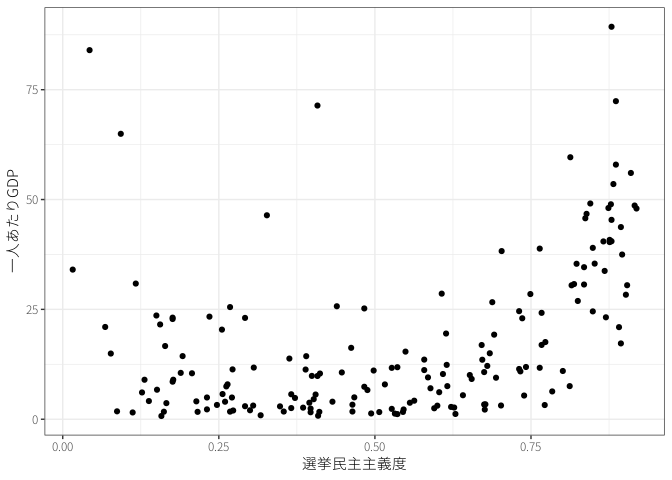
\includegraphics{human_rights_files/figure-pdf/unnamed-chunk-2-1.png}

}

\caption{自由権保障の推移}

\end{figure}

\begin{figure}[htpb]

{\centering 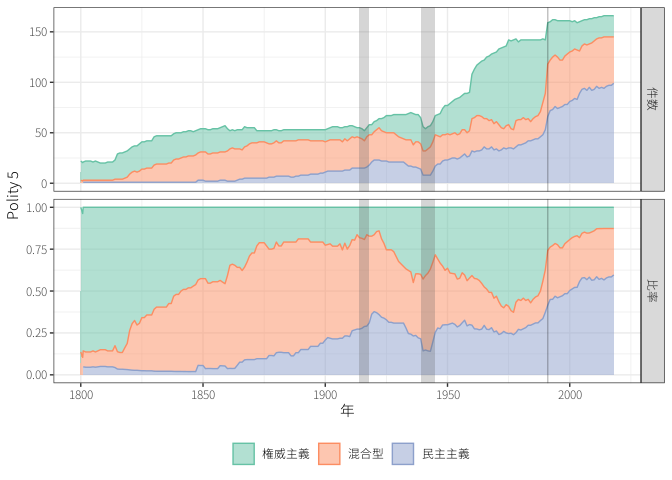
\includegraphics{human_rights_files/figure-pdf/unnamed-chunk-3-1.png}

}

\caption{自由権保障の水準}

\end{figure}

\hypertarget{ux4ebaux6a29ux4fddux969cux3092ux5de1ux308bux653fux6cbb}{%
\section{人権保障を巡る政治}\label{ux4ebaux6a29ux4fddux969cux3092ux5de1ux308bux653fux6cbb}}


\renewcommand\refname{戦争と人権}
  \bibliography{references.bib}


\end{document}
